% !TeX root = ../../thesis.tex

\section{Neither Secure Boot nor BitLocker}

We start by implementing a baseline attack, that we can use to test against Secure Boot and BitLocker and further build upon.
The implementation in the form of a bootkit and a rootkit both share the same approach and core functionality.
The general approach of our attack is to access the Windows installation from within \ac{UEFI} environment and gain elevated code execution by modifying its contents.

\subsection{Bootkit}
\label{sec:attacks:neither:bootkit}

We start with the bootkit.

\subsubsection{Infection}

We have two ways to infect a system, we can either use a bootable medium such as a CD-ROM or \ac{USB} stick with a \ac{UEFI} application installing the bootkit or using a Windows executable.
Booting into the installer application requires either the firmware implementation or the boot order to prefer booting from the removable media over Windows.
This can be forced when booting accessing the interactive firmware menu at startup, given that it is not password protected.
Installation from Windows requires admin privileges to mount and modify the \ac{ESP}.

The installation process is identical for both options, we access the \ac{ESP} and create a copy of the Windows Boot Manager located under \program{EFI\textbackslash Microsoft\textbackslash Boot\textbackslash bootmgfw.efi}.
We then replace the original with our bootkit as well as dropping all resources required by the bootkit on the \ac{ESP}.
Now that our bootkit is in place of the Windows Boot Manager, when the \ac{UEFI} Boot Manager selects the boot load option for the Windows Boot Manager, it will cause our bootkit to be executed.
\autoref{fig:windows-boot-entry} shows a dump of the Windows boot entry using the \ac{UEFI} shell command \program{bcfg}.
The entry contains the device path including the file path and optional data.

\begin{figure}[htb]
    \centering
    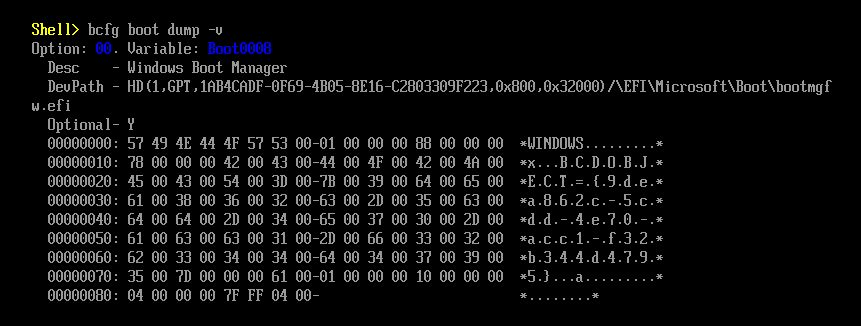
\includegraphics[width=1.0\textwidth]{attacks/neither/windows_boot_entry.png}
    \caption{Windows boot entry, part of the \ac{UEFI} shell output of \program{bcfg}}
    \label{fig:windows-boot-entry}
\end{figure}

\subsubsection{File access}

The most important step for a storage-based approach is gaining access to the Windows installation from within the \ac{UEFI} environment.
Since \ac{UEFI} does not require the firmware to come with an \ac{NTFS} driver, our attack has to come with its own.
\ac{EDK} II does not provide one, but we can use the open source \ac{NTFS} driver \program{ntfs-3g} from Tuxera \cite{ntfs-3g}.
It was ported to the \ac{UEFI} environment by \emph{pbatard} \cite{ntfs-3g-uefi}.
Using \ac{EDK} II to compile it, we receive a \program{.efi} executable image.

We can use the \ac{UEFI} shell and its file system related commands to test the \ac{NTFS} driver's capabilities.
When booting into the \ac{UEFI} shell we are greeted with a screen displaying the \ac{UEFI} specification version the firmware supports and a list of default mappings for file systems and block devices.
These mappings are created by the shell to provide a short name that can be used interchangably with longer device path when issuing commands \cite[Section 3.7.2]{uefi-shell-spec}.
They are designed to be consistent across reboots as long as the hardware configuration stays the same and are comparable to Windows partition letters \cite[Appendix A]{uefi-shell-spec}.
\autoref{fig:mapping} shows the mapping of a partition containing a Windows installation.
As there is no \ac{NTFS} driver present yet, it is only displayed as a block device.

\begin{figure}[htb]
    \centering
    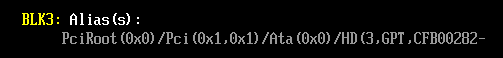
\includegraphics[width=0.8\textwidth]{attacks/neither/mapping}
    \caption{Mapping of the Windows parition}
    \label{fig:mapping}
\end{figure}

We can enter the mapping name of the file system containing our \ac{NTFS} driver to use it as our current working directory and load the driver using the \program{load} command.
The command is executed successfully and can the driver is now listed when querying the currently loaded drivers with the command \program{drivers}.
We can now instruct the default mappings to be reset with the \program{map -r} command, to receive an updated list including the file systems now provided through the \ac{NTFS} driver.
\autoref{fig:mapping-ntfs} also shows us that the new file system now sits on top of a device which previously was only listed as a block device.

\begin{figure}[htb]
    \centering
    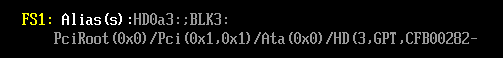
\includegraphics[width=0.8\textwidth]{attacks/neither/mapping_ntfs}
    \caption{Mapping of the mounted Windows parition}
    \label{fig:mapping-ntfs}
\end{figure}

As done before we now type the mapping name of the new file systems, we check the root directories' contents with \program{ls} until we find the partition containing the Windows installation and then enter \program{vol} to check the access rights.
This reveals that the file system is currently read\-/only.
Upon debugging the \ac{NTFS} driver it appears to be that the driver falls back to read\-/only when it encounters a file that indicates that the Windows system is in hibernation mode.
We can remove this fallback from the \ac{NTFS} driver's code and recompile.


\begin{figure}[htb]
    \centering
    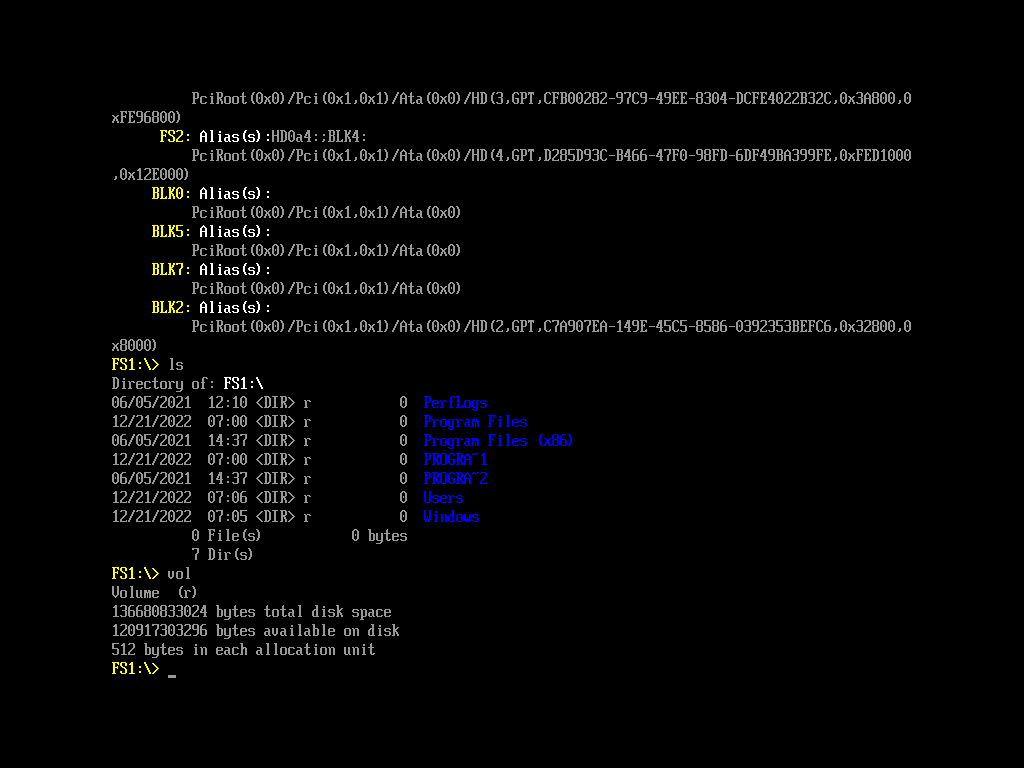
\includegraphics[width=0.5\textwidth]{attacks/neither/vol}
    \caption{Volume Information of the Windows File System}
    \label{fig:mapping-ntfs}
\end{figure}

On our hardware setups we noticed that the firmware can already ship with an \ac{NTFS} driver included, which is read\-/only.
In the case of our rootkit we would be able to remove this driver by modifying the firmware iamge, but we can implement a solution that applies to both types of \ac{UEFI} payload.
We can change the \ac{NTFS} driver to install its \hyperref[lst:simple-file-system-protocol]{Simple File System Protocol} under a \ac{GUID} different to the regular \code{gEfiSimpleFileSystemProtocolGuid}.
This makes it possible to install two instances of the \hyperref[lst:simple-file-system-protocol]{Simple File System Protocol} alongside each other on the same controller.
The alternative \ac{GUID} can then searched for by our root- and bookit, to retrieve our specific protocol instance with write access.
The driver also has to open the protocols it uses without demanding exclusive ownership over them.
This prevents the \ac{NTFS} driver from being when denied access, when trying to open a protocols that is already in exclusive ownership \cite[Section 7.3]{uefi-spec}, which would be a likely occurrence as filesystem drivers are encouraged to get exclusive control over their block device \cite[Section 13.5]{uefi-spec}.

We now know that, provided we get to load the \ac{NTFS} driver, we can read and write the files of a Windows installation.
Thus we drop the driver together with the bootkit onto the \ac{ESP} as part of our infection process.
When our bootkit is executed, we use the \hyperref[lst:loaded-image-protocol]{Loaded Image Protocol} of our own image handle to retrieve the source device handle, our bootkit was loaded from \cite[Section 9.1]{uefi-spec}.
As both files reside within the same volume, we can use this handle to call the boot services \code{LoadImage} and \code{StartImage} to execute the driver.
Since the driver conforms to the \ac{UEFI} Driver Model, we also need to connect the driver to device representing the Windows parition using the \hyperref[lst:driver-binding-protocol]{Driver Binding Protocol}.
We can do this by retrieving all protocol instances and iterating over all controllers, to connect them recursively.
This way so the driver can assume controller over all \ac{NTFS} formatted volumes and install an instance of \hyperref[lst:simple-file-system-protocol]{Simple File System Protocol} on their handles.

\subsubsection{Payload deployment}

Before we can deploy our payload we first need to read it into memory.
\code{LoadImage} is reserved to be used for \ac{UEFI} images, non\-/executable files are read directly with the \hyperref[lst:simple-file-system-protocol]{Simple File System Protocol}.
The \ac{ESP}'s device handle can be used with the boot service \code{HandleProtocol} to retrieve its instance of the \hyperref[lst:simple-file-system-protocol]{Simple File System Protocol}.
A call to \lstinline{OpenVolume} results in an instance of the \hyperref[lst:simple-file-system-protocol]{File Protocol} representing the root folder of the volume \cite[Section 13.4]{uefi-spec}.
The root directory can then be used to open and read our payload with an absolute path.

To perform the write operation we need the device handle of the volume containing the Windows installation.
We can use the boot service \code{LocateHandleBuffer} to receive an array of all handles that support the \hyperref[lst:simple-file-system-protocol]{Simple File System Protocol}, this includes volumes such as the Windows recovery partition or the \ac{ESP} we just used.
We can iterate over all handles and search for the Windows folder to identify the correct volume.

Now the question arises as to where we write our payload to, our goal is automatic and elevated execution.
\emph{MosaicRegressor} writes its payload to the Windows startup folder, a folder whose contents are automatically executed at system startup.
The programs within the startup folder are unfortunately not automatically run at an elevated level, so this isn't a suitable target location.
We also cannot trivially overwrite or modify executables that are part of the Windows startup process, as \ac{KMCI} will verify their code integrity before execution.

Our approach is to use the Task Scheduler.
The Task Scheduler is a Windows service responsible for managing the automatic execution of background tasks \cite[Section 10]{windows-internals-7-part2}.
Tasks are performed on certain triggers, which may be time-based (periodically or on a specific time) or event-based, for example on user logon or system boot \cite{microsoft-task-scheduler-triggers}.
A task can perform various actions upon invocation \cite{microsoft-task-scheduler-actions}, we will focus on command execution.
Most tasks will simply execute other programs as their action, this execution is performed under specified a security context \cite{microsoft-task-scheduler-security-contexts}.
The idea is to have a task, that performs its action with a high privilege level, execute our payload.
The task of our choosing is called \program{Proxy} and found under the \program{Autochk} folder, its properties can be seen in \autoref{fig:proxy}.

\begin{figure}[htb]
    \centering
    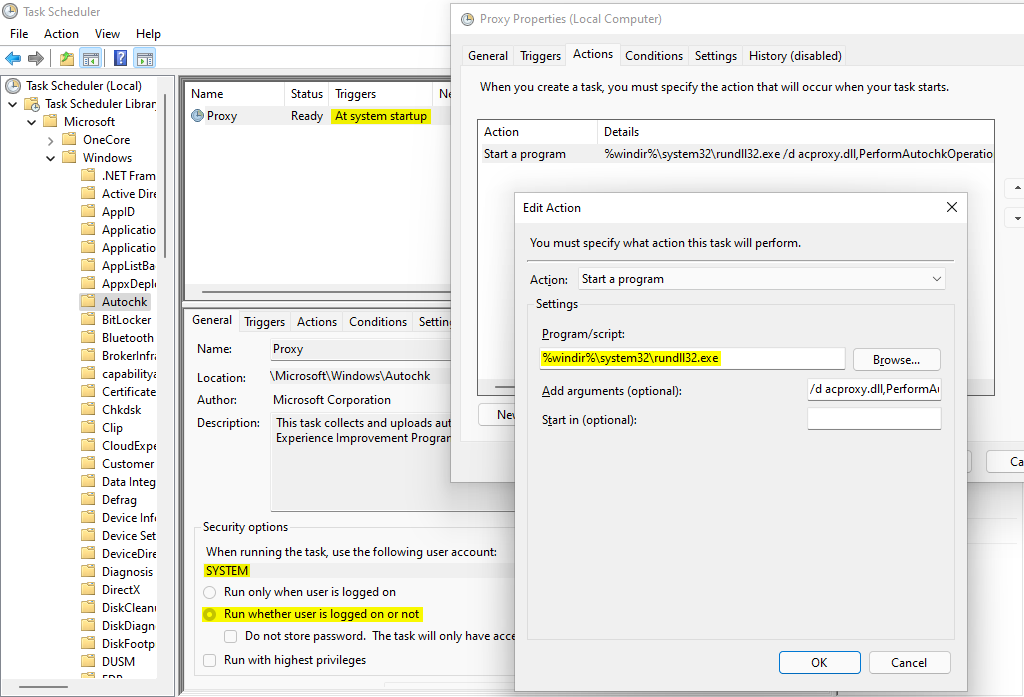
\includegraphics[width=1.0\textwidth]{attacks/neither/proxy}
    \caption{\program{Proxy} Task shown using the Task Scheduler Configuration Tool}
    \label{fig:proxy}
\end{figure}

The \program{Proxy} task is triggered at system startup (with a 30 minute delay) and its action is to start the program \program{rundll32.exe} with the options \code{/d acproxy.dll,PerformAutochkOperations}.
This causes \program{rundll32.exe} to load the \program{acproxy.dll} \ac{DLL} into memory and invoke its exported function \code{PerformAutochkOperations()} \cite{microsoft-rundll32}.
The function name as well as the task name suggest the performed action relates to the Windows utility \program{autochk} which verifies the integrity of \ac{NTFS} file systems \cite{microsoft-autochk}.
Under security options we can see, that the task is executed using the built\-/in \emph{SYSTEM} account.
Over all this task is the perfect candidate to run our payload.

The Task Scheduler keeps book of its active tasks in the registry under \program{HKLM\textbackslash SOFTWARE\textbackslash Microsoft\textbackslash Windows NT\textbackslash CurrentVersion\textbackslash Schedule\textbackslash TaskCache}.
The tasks are grouped by four subkeys \program{Boot}, \program{logon}, \program{plain} and \program{Maintenance}.
The entries under these subkeys consist only of a \ac{GUID}, the \ac{GUID} references the task descriptors that are saved using task master (registry) keys, these task master keys are located under \program{HKLM\textbackslash SOFTWARE\textbackslash Microsoft\textbackslash Windows NT\textbackslash CurrentVersion\textbackslash Schedule\textbackslash TaskCache\textbackslash Tasks} \cite[Section 10]{windows-internals-7-part2}.
There also exist a secondary copy of the task descriptors, on the regular file system under \program{\%windir\%\textbackslash system32\textbackslash Task}, stored as \ac{XML} files.

We can use the Task Scheduler Configuration Tool to modify the \program{Proxy} task on a system under our control, changing the executable path as well as remove the delay configured in its trigger.
To verify the privileges our payload is executed with, we can save the output of \program{whoami /all} into a file.
The \program{whoami} command shows the current user and privileges \cite{microsoft-whoami}.
After manually triggering the task through the configuration tool, we see that our payload was run from the \emph{nt authority\textbackslash system} user account, which is the most privileged system account \cite{microsoft-localsystem-account}.

\TODO{whoami /all snippet}

With the Windows registry editor \program{reged.exe} we can navigate to the task descriptor store and search for the task master key belonging to our task.
We can then export the task master key and import it on our victim's system as part of our attack.
By importing an entire registry key, instead of modifying a single value of an existing registry key, the victim's registry keys maintains their integrity, as with a full overwrite the registry key's hash value is also changed.
To import the key we can use a Linux utility called \program{chntpw} whose primary purpose it is to reset the password of local Windows user accounts \cite{chntpw}.
It does this by editing the hive files of a Windows installation and as such the author also offers a standalone registry editor called \program{reged}.
We can test the Linux tool when dual\-/booting Linux and Windows.
For now we place our payload manually in the Windows installation and then boot into Linux, where we can open the \program{HKEY\_LOCAL\_MACHINE/SOFTWARE} hive in \program{reged} and import our modified registry key.
This overwrites the task descriptor and when booting into Windows our payload is executed.

\TODO{starts here}

The next step is to port the \lstinline{reged} utility so that it works in the UEFI environment, so we can use it as part of our bootkit.
% most stdlib stuff is just mapping to UEFIlib stuff with equivalents or using gcc implementations
The porting process boils down to providing semantically equivalent definitions of external function calls, such as c standard library and Linux kernel functions, to link against.
Declarations and macros are still supplied by the local compiler's system headers.
Function definitions can often be translated to \ac{UEFI} equivalents, \ac{EDK} II has libraries offering implementations of commonly used abstraction.
% memory allocation (malloc, calloc, realloc), memory manipulation (memset, memcpy) string manipulation (sscanf, strtol), stdout (printf), abort, exit
Memory allocation maps to the MemoryAllocationLib, memory manipulation to BaseMemoryLib, basic string manipulation to BaseLib, stdout to PrintLib (only relevant for print debugging).
% cstdio is non trivial and has to be implemented by calling protocols on the right volume
Function calls related to standard input and output such as opening, reading and writing a file, namely the hive file, are more complex and have to be mapped to the \ac{UEFI} protocols \hyperref[lst:simple-file-system-protocol]{Simple File System Protocol} and \hyperref[lst:simple-file-system-protocol]{File Protocol}.
Luckily the author of \lstinline{reged} used distinct functions to access the hive file and registry file, making it possible to keep the original source code unmodified, except for a change in the import behavior.
The name of a task master key is the task's \ac{GUID}, which may differ from device to device, thus we cannot import a key into its exact path, we instead iterate over the subkeys of the target's parent key.
We then match for the name value of the key.

Now that we modified the Windows installation to execute our payload upon boot, we need to transfer execution from the bootkit to the original Windows Boot Manager.
Loading the original application is inspired by how the UEFI Boot Manger loads boot options, this includes relaying the \lstinline{LoadOptions} and \lstinline{ParentHandle} of the \emph{\ac{EFI} Loaded Image Protocol} \cite[Section 9.1]{uefi-spec} instance installed to our bootkit to the Windows Boot Manager.

\TODO{ends here}


\subsection{Rootkit}

Performing the attack in the form of a rootkit is very similar and mainly differs in the infection process.
The \ac{UEFI} payload is now compiled as a \ac{DXE} driver instead of a regular \ac{UEFI} application.
When it is placed in a \ac{DXE} volume it is automatically loaded by the \ac{DXE} Dispatcher iterating over the \ac{FV}, loading  drivers whose dependencies are resolved.
The core functionality of our \ac{UEFI} payload is identical with the exception that we don't have to manually load the \ac{NTFS} driver anymore and accessing the Windows payload is now done with the \emph{Firmware Volume2 Protocol} defined in the \cite[Section 3.4.1]{pi-spec}, instead of \emph{Simple Filesystem Protocol}.
There are no traditional file names in a \ac{FFS}, and we have to search for files using the files's \acp{GUID}, which is read from the \ac{EDK} II module file.

\subsubsection{Infection}

Infection with the rootkit is has a much higher barrier of entry, as it requires read and write access to the firmware image.
\autoref{sec:test-setup} lists how we access the firmware images on our target systems.
\TODO{MEEE}
But there are also other ways to do this, \autoref{sec:past-threats} vector\-/edk potentially exploit \ac{OEM} specific flash mechanism, signing with stolen private key, part of the supply chain, might also be physical \TODO{LIST ALL OPTIONS}

We we are in possession of the image, we need to insert our payload into a \ac{DXE} volume and redeploy the modified image.
We can do this using \program{UEFITool}, where we navigate to a \ac{DXE} volume, they are identified by containing \ac{DXE} drivers.
On our \autoref{sec:test-setup:lenovo} system the firmware image did not contain enough free space to allow for the addition of our payload.
By deleting network related drivers

We cannot directly drop our \ac{UEFI} payload in form of \lstinline{.efi} files with UEFITool, because \ac{DXE} drivers have three mandatory sections: the \ac{PE32} executable section, composed of the \lstinline{.efi} file content, a version section and the \ac{DEPEX} section \cite[Vol. 3, 2.1.4.1.4]{pi-spec}.
% compile dxe driver within ovmf
% generate unused volume to receive .ffs file with version, depex, user interface and pe section
For our \ac{UEFI} payload to be generated as a sectioned \ac{FFS} file we add our files to the build process of \ac{OVMF} package in \ac{EDK} II. When part of the \ac{FDF} which is used to generate a firmware image file, the intermediary \lstinline{.ffs} files from the build process are of much value for us.
% pack executable binary as uefi module
% EDK II produces freeform image with one raw section
For our Windows payload we can use a special \ac{EDK} II module type which takes binary files as input, resulting in a sectioned file of type \lstinline{EFI_FV_FILETYPE_FREEFORM}, with no restrictions on the contained file sections \cite[Vol. 3, 2.1.4.1.7]{pi-spec}.
The output contains only one file section of type \lstinline{EFI_SECTION_RAW} consisting of the binary payload.
This use of this special module has the benefit that its \ac{GUID} is used to attribute the sectioned file when being placed in the firmware volume.
Not that we have \lstinline{.ffs} files corresponding to all our resources used in the attack we can import these into the target image with UEFITool.

\TODO{this}
overwrite the SPI flash with modified image by using the programmer again.

\clearpage
